

\usetikzlibrary{arrows.meta,decorations.pathmorphing}


\begin{frame}{system call process}
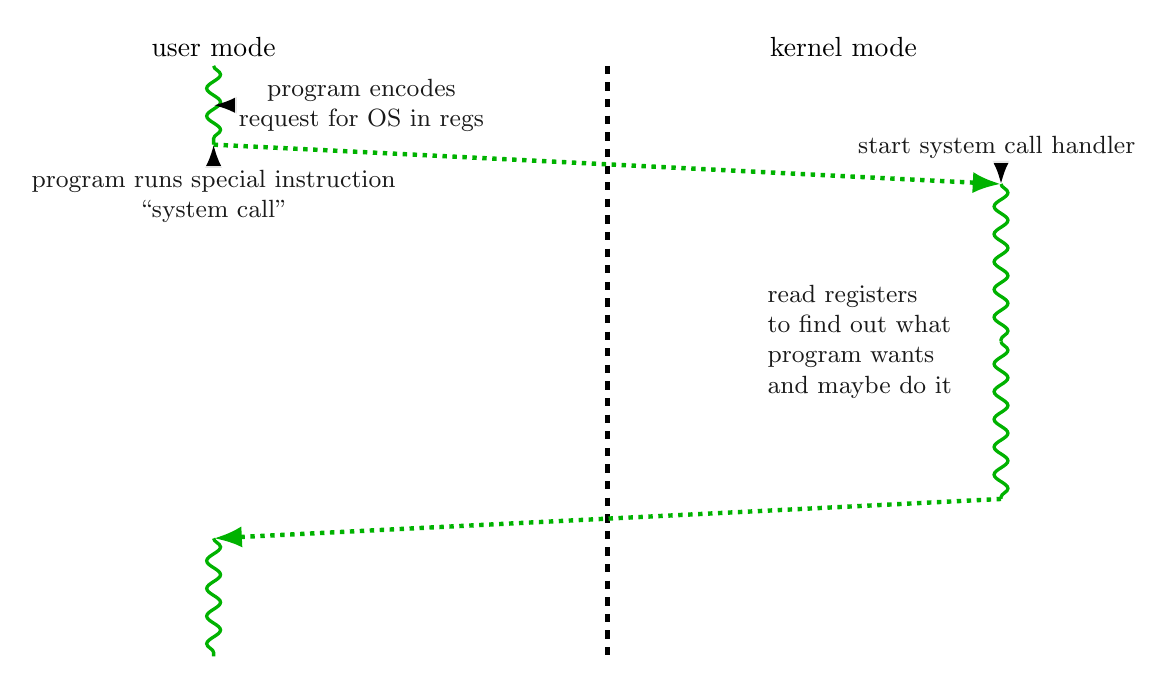
\begin{tikzpicture}
\draw[ultra thick,dashed] (1, -.5) -- (1, -8);
\begin{scope}[every node/.style={anchor=south,align=center}]
    \node at (-4, -.5) {user mode};
    \node at (4, -.5) {kernel mode};
\end{scope}
%\draw[thick,dotted] (-7, -4) -- (7, -4);
\tikzset{
    snake/.style={very thick,decorate,decoration={snake}},
    >=Latex,
    process A/.style={green!70!black},
    OS code/.style={blue!70!black},
},
\draw[snake,process A] (-4, -.5) -- (-4, -1.5) coordinate (before enter kernel);
\draw[snake,process A] (6, -2) coordinate (after enter kernel) -- (6, -4) coordinate (before swtch);
\draw[snake,process A] (6, -4) coordinate (after swtch) -- (6, -6) coordinate (before exit kernel);
\draw[snake,process A] (-4, -6.5) coordinate (after exit kernel) -- (-4, -8);
\draw[process A,ultra thick,->,dotted] (before enter kernel) -- (after enter kernel);
\draw[dotted,very thick,<-] ([yshift=0.5cm]before enter kernel) -- ++(.25cm, 0cm) node[right,align=center,font=\small,fill=white,fill opacity=0.9, inner sep=0.5mm] {
    program encodes \\ request for OS in regs
};
\draw[dotted,very thick,<-] (before enter kernel) -- ++(0cm, -.25cm) node[below,align=center,font=\small,fill=white,fill opacity=0.9, inner sep=0.5mm] {
    program runs special instruction \\
    \myemph{``system call''}
};
\draw[dotted,very thick,<-] (after enter kernel) -- ++(0cm, .25cm) node[above,align=center,font=\small,fill=white,fill opacity=0.9, inner sep=0.5mm] {
    start system call handler
};
%\draw[ultra thick,->,in=145,out=145] (before swtch) to (after swtch);
\node[align=left,font=\small,fill=white,fill opacity=0.9,anchor=east] at (5.5, -4) {
    read registers \\
    to find out what \\
    program wants \\
    and maybe do it 
};
\draw[process A,ultra thick,->,dotted] (before exit kernel) -- (after exit kernel);
%\draw[dotted,very thick,<-] (before exit kernel) -- ++(0cm, -.25cm) node[below,font=\small,fill=white,fill opacity=0.9, inner sep=0.5mm,align=center] {
%    exit system call handler
%};
\end{tikzpicture}
\end{frame}

